\documentclass{tufte-handout}

\title{On ultimate; O1: primary middle, left wing}
\author[James Reynolds]{James Reynolds}

%\date{28 March 2010} % without \date command, current date is supplied

%\geometry{showframe} % display margins for debugging page layout

\usepackage{graphicx} % allow embedded images
  \setkeys{Gin}{width=\linewidth,totalheight=\textheight,keepaspectratio}
  \graphicspath{{graphics/}} % set of paths to search for images
\usepackage{amsmath}  % extended mathematics
\usepackage{booktabs} % book-quality tables
\usepackage{units}    % non-stacked fractions and better unit spacing
\usepackage{multicol} % multiple column layout facilities
\usepackage{lipsum}   % filler text
\usepackage{fancyvrb} % extended verbatim environments
  \fvset{fontsize=\normalsize}% default font size for fancy-verbatim environments

% Standardize command font styles and environments
\newcommand{\doccmd}[1]{\texttt{\textbackslash#1}}% command name -- adds backslash automatically
\newcommand{\docopt}[1]{\ensuremath{\langle}\textrm{\textit{#1}}\ensuremath{\rangle}}% optional command argument
\newcommand{\docarg}[1]{\textrm{\textit{#1}}}% (required) command argument
\newcommand{\docenv}[1]{\textsf{#1}}% environment name
\newcommand{\docpkg}[1]{\texttt{#1}}% package name
\newcommand{\doccls}[1]{\texttt{#1}}% document class name
\newcommand{\docclsopt}[1]{\texttt{#1}}% document class option name
\newenvironment{docspec}{\begin{quote}\noindent}{\end{quote}}% command specification environment

\begin{document}

\maketitle% this prints the handout title, author, and date


\begin{marginfigure}%
  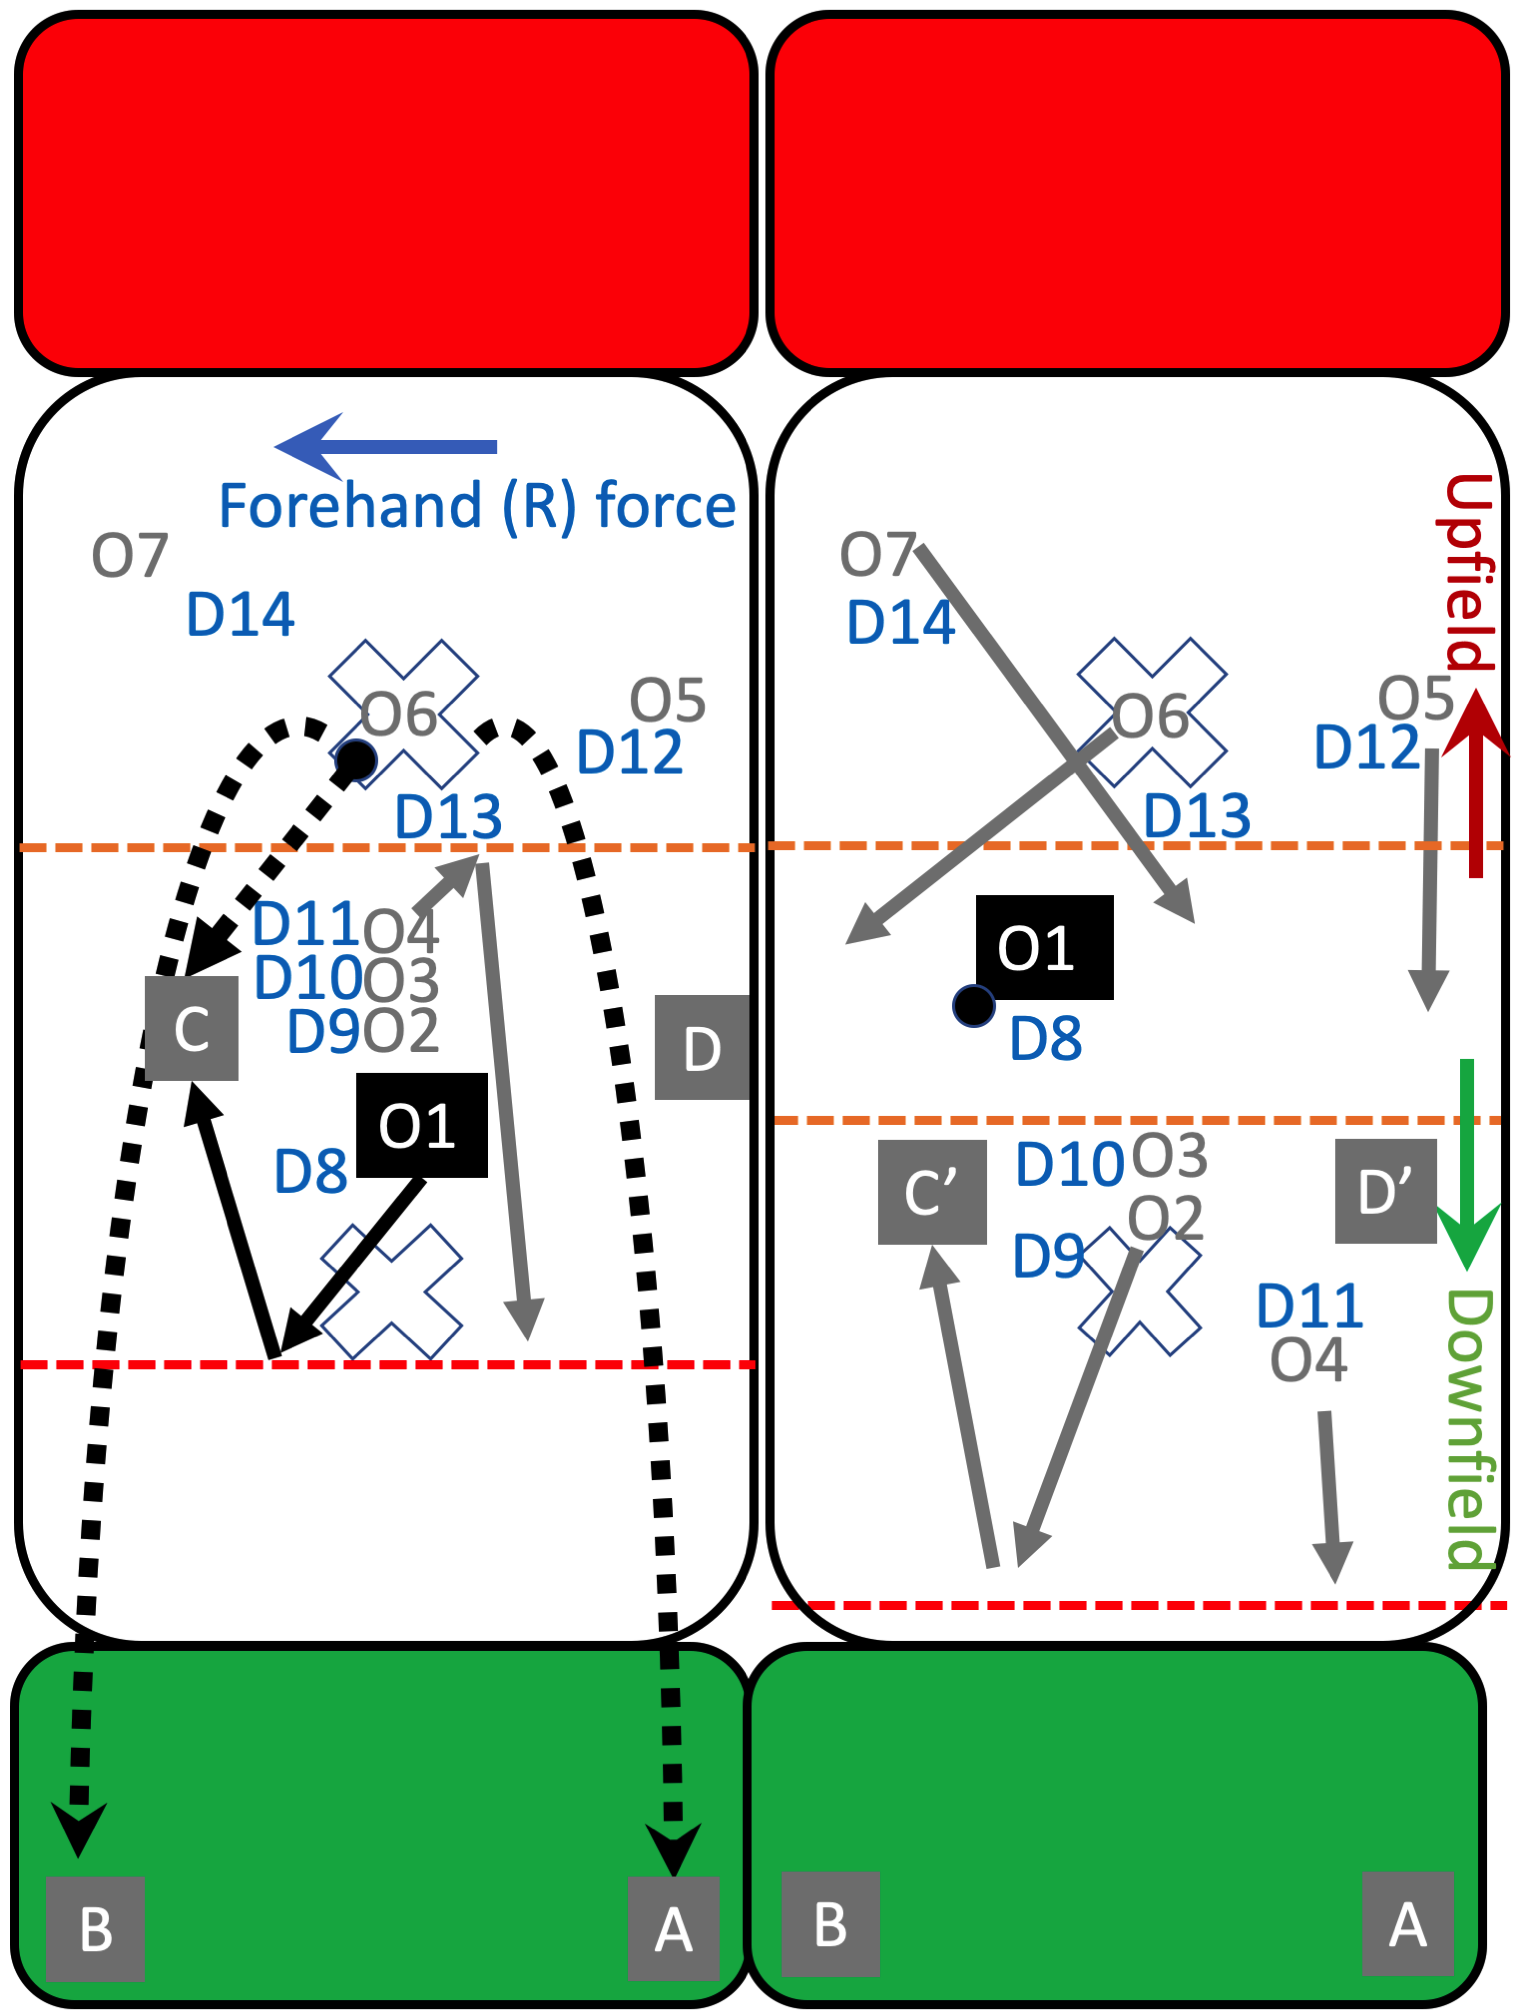
\includegraphics[width=\linewidth]{O1-vertical}
  \caption{Vertical stack formation}
  \label{fig:O1-vertical}
\end{marginfigure}



%\printclassoptions
This document is about 
playing primary 'middle' 
or left wing 
on offence,
referred to here 
as position O1\footnote{This
is part of a series, 
available at
\url{https://github.com/James-Reynolds/Ultimate-strategy-and-tactics}}.
You are starting the point on offence. 
Let the handlers 
deal with catching the pull, but
as you run downfield
try to figure out 
what defence structure
is being used. 
%\footnote{It could be:
%person-match defence,
%person-match-last-back-helps,
%person-match-with-a-poacher,
%person-match-with-lots-of switching,
%force-middle,
%force-straight-up,
%zone-3-3-1-force-middle-
%zone-3-3-1-force-sideline
%zone-3-3-1-force-forehand
%zone-3-3-1-force-backhand
%zone-3-3-1-etc
%zone-3-2-2, 
%zone-2-3-2, 
%zone-1-3-2-1 (puppy-fence),
%clam,
%or something else}.

\section{Person-match defence: vertical stack}\label{sec:vertical}

Figure \ref{fig:O1-vertical} shows 
how everyone might 
setup 
if there is a brick called,
a forehand force, 
person-match defence, 
and a vertical stack.


Restricting your cutting 
to between 
the dashed 
horizontal 
lines 
can help\footnote{
Position of 
the dashed red line might vary
with how far O6 
can or will 
throw. 
Note also how in 
Figure \ref{fig:O1-vertical2} 
these lines move, 
as the disc moves.}. 
If you go 
downfield of the dashed red line 
before the disc is in the air,
D8 may be able 
get to
A or B 
before the disc,
intercepting 
or preventing 
deep throws to 
you or others. 
Similarly, 
if you go 
upfield of the dashed yellow line
then D8 may 
be able to help
prevent dump throws from O6
to O5 
or O7.
Hence,
if you cut to C
but the disc is not thrown to you
perhaps cut deep 
to clear the area, 
then return to the stack
and make space for O2-O4. 


O6 is shown
potentially throwing 
you (O1) either:
\begin{enumerate}
\item A break-side 
huck to A.
This throw is 
probably 
difficult. 
However, you as O1
can just
stand still 
till O6 throws it, 
then run and catch it.
Figure \ref{fig:O1-vertical} indicates how 
D8 will be on the wrong side of you
and so probably 
be able to get to the disc
first.
\item An open-side huck to B. 
This is viable if: 
D8 is closer to the disc than you; 
you are faster than D8; or 
D8 does not cover 
an initial cut downfield (black arrow). 
\item A throw 
to C.
The solid black arrows indicate 
a cut you might do;
initially going deep,
but then coming back-under
on the open side.
\end{enumerate}

\begin{marginfigure}%
  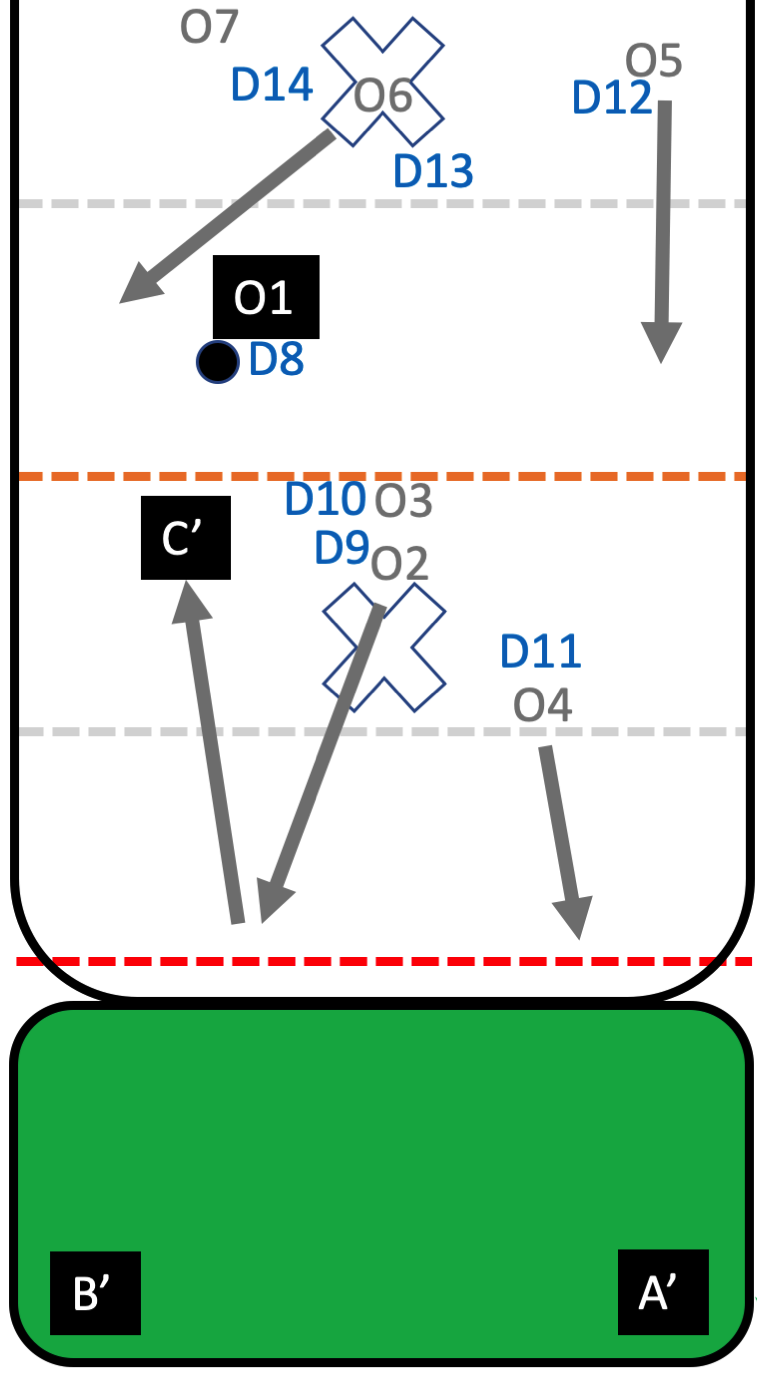
\includegraphics[width=\linewidth]{O1-vertical2}
  \caption{Vertical stack progression}
  \label{fig:O1-vertical2}
\end{marginfigure}


Figure \ref{fig:O1-vertical2} shows 
the disc having been thrown to you
on the back-under cut towards C. 
In order of desirability, 
your options may include: 
(1)
off-load to O6, 
putting them in power position;
(2) throwing to A' to hit O2 or O4;
(3) throwing to B' or C' for O2;
(4) break force throw 
to centre the disc
to O3 or O5;
(5) dump to O7.
Then, head back to the stack, 
or make another cut.

Vertical stack is effective
 against other forms of person-match defence, 
although some adjustments may be needed. 
For example, 
%against (1) RH-backhand-force: mirror the above.
against (1) person-match-straight-up-force: 
hucks are likely harder, 
but your defender (D8) 
may just cover you under. 
Hence, maybe just
stand still as the handlers 
move it around until
they can send it deep.
Otherwise, 
maybe cut out to the sidelines.
Against (2) person-match-with-lots-of-switches: 
maybe switch
 to a horizontal stack\footnote{
Or coordinate 
with O2 to both
go downfield 
to overload D8, 
or both go upfield to overload D9.}.
%Against (3) person-match-force-middle: 
%it may be difficult to throw to under cuts, 
%so maybe wait for a throw deep 
%(going over the stack) 
%to the opposite side of the
%field from the thrower. 
%Against (4) person-match-last-player-back-covers-deepest: 
%maybe coordinate with O2 
%so that you both go deep at the same time, 
%one to A and 
%one to B.
%D8 may then have to choose 
%which of you to cover.  
%You might also 
%coordinate you back-under cuts 
%to overload D9.}.


\begin{marginfigure}%
  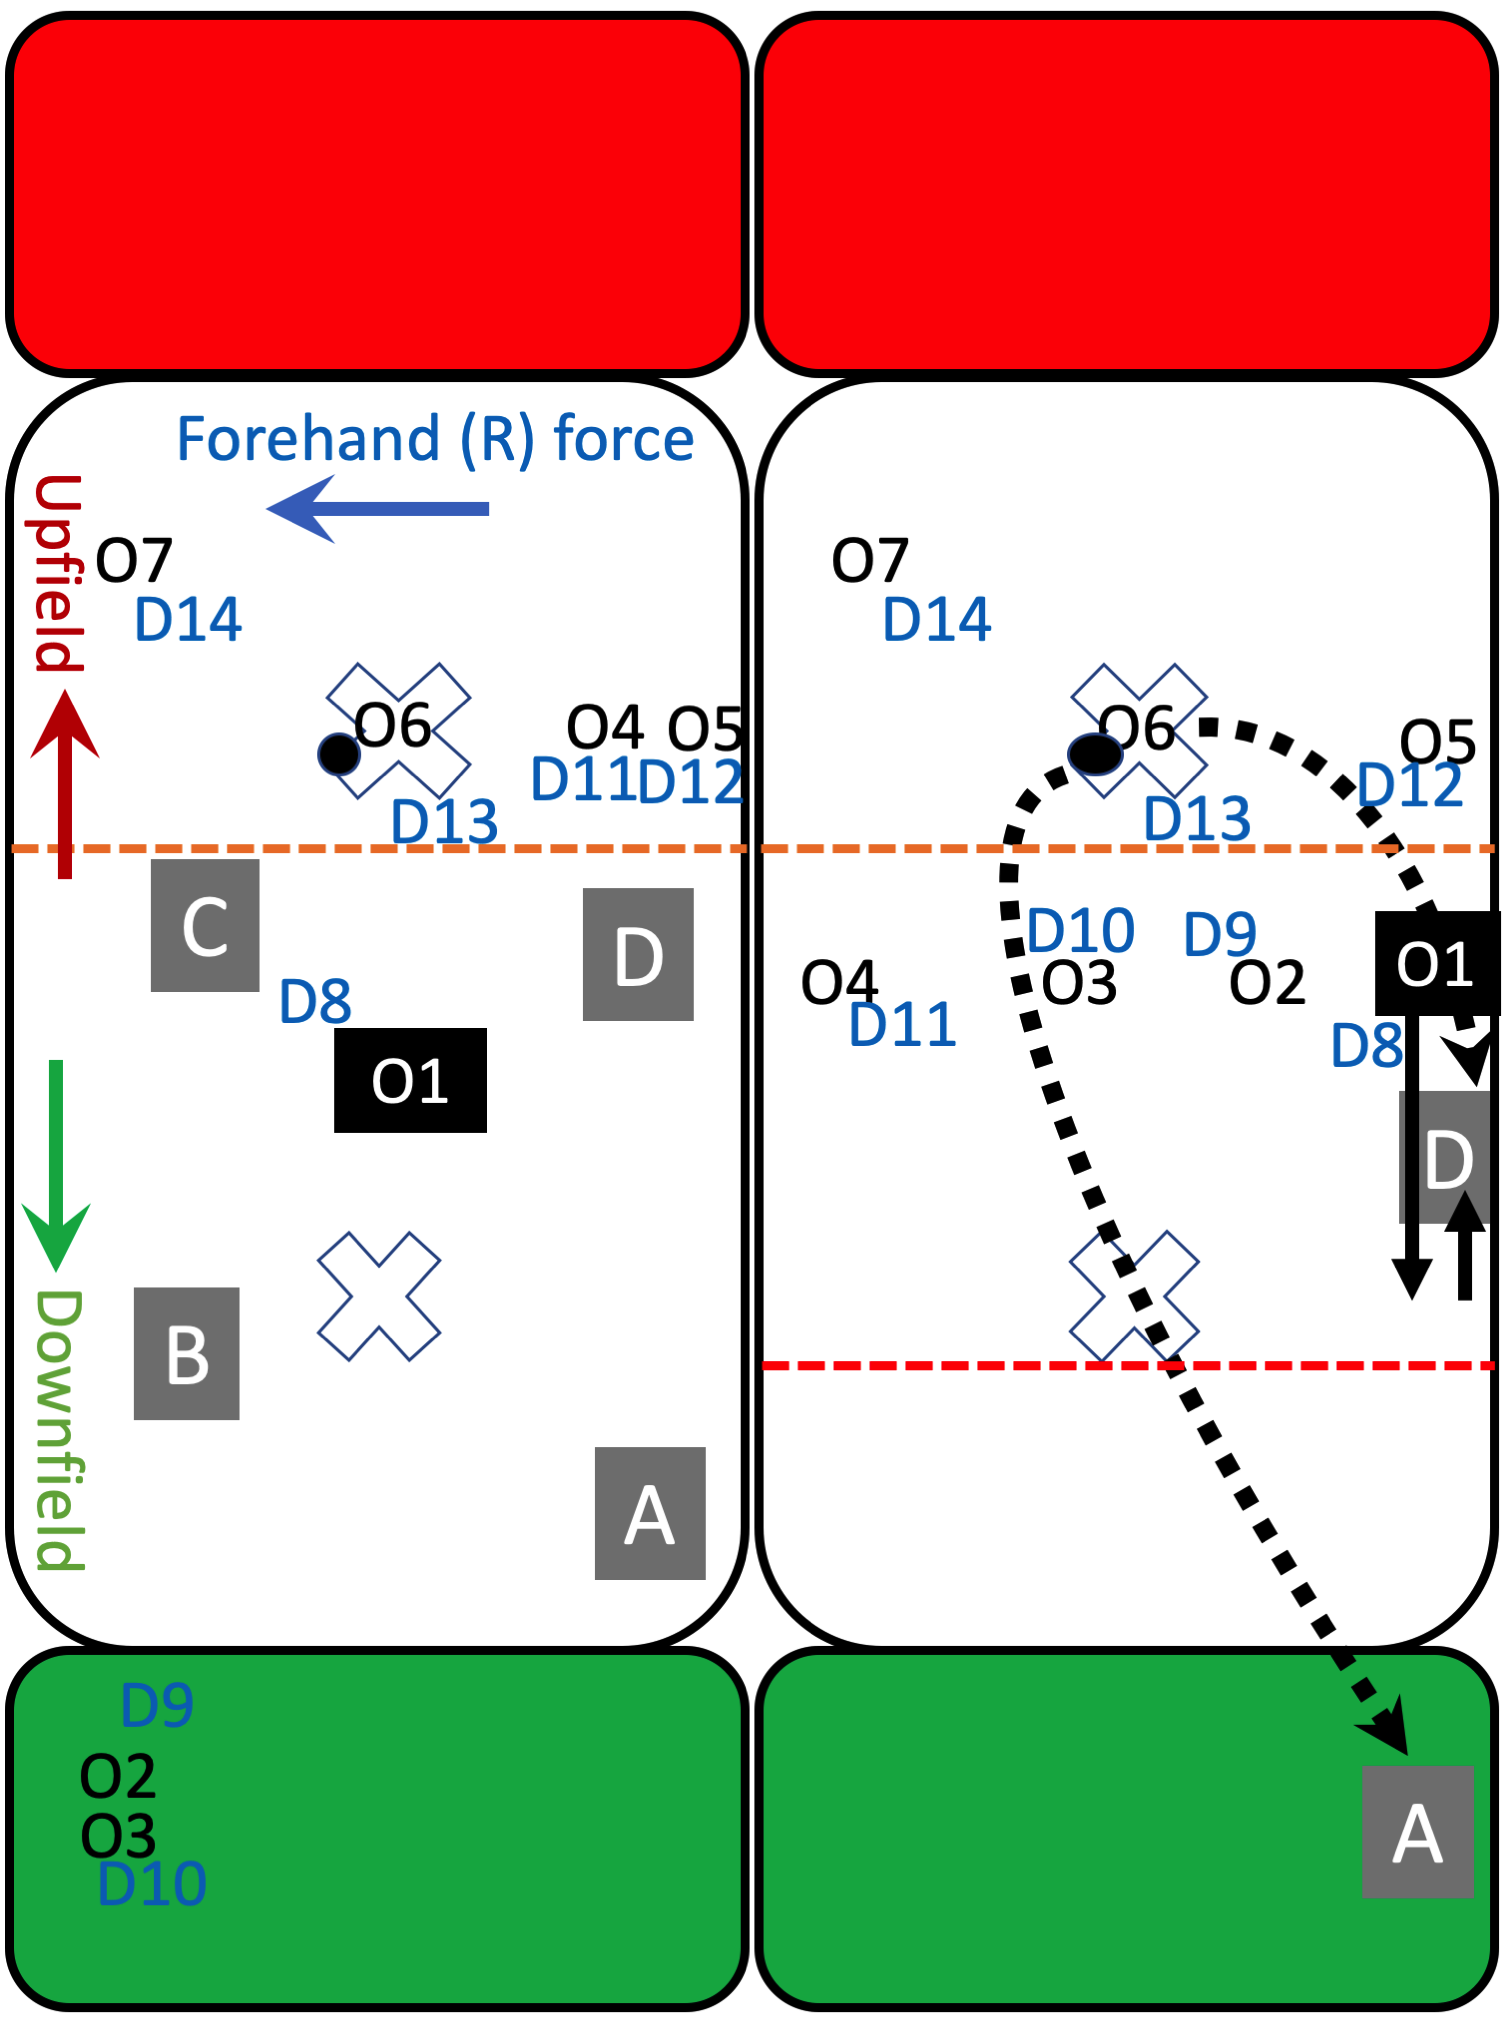
\includegraphics[width=\linewidth]{O1-horizontal}
  \caption{Horizontal stack formation}
  \label{fig:O1-horizontal}
\end{marginfigure}


\subsection{Person-match defence: horizontal stack}\label{sec:horizontall}
In a horizontal stack 
the strategy is to cut 
upfield and downfield (black arrows)
within your quarter of the field\footnote{
Other cuts
can work. 
For example, 
diamond cuts 
involve trading places 
with your neighbour
(02). 
However, this may need
coordination. 
So maybe keep it simple 
and just stay on the wing?}. 
Figure \ref{fig:O1-horizontal} shows 
O1 on the left wing. 
O6 
can potentially 
throw to you 
at A 
or D\footnote{
The black arrows
show a back-under cut 
opens space 
for this throw.}. 
If you get the disc 
at D 
a huck to 
A for O2 or 
to B for O4 
may be effective 
if thrown as 
a (RH) outside-in backhand or
inside-out forehand 
(to the break-side of your receivers). 
But if that is not on, 
it is probably best 
to move it 
back to the middle of the field 
via a dump to O5 or O6. 

However, 
from the starting position,
O6 throwing to 
O2, O3 or O4 will probably 
be easier. 
Hence, rather than cutting immediately, 
you may wish to 
wait and 
cut for a throw from someone else. 

A typical pattern
is that D8 will
help D9, D10 and D11 
by poaching deep\footnote{
Person-match-but-last-person-covers-deep defence}. 
To beat this: 
stay still 
on the left wing,
so O6 can throw it 
straight to you. 
Alternatively: 
O6 might dump to O5 who can then throw to you;
you can trade spots with O5;
or you can moving across to the open side, 
between D10 and O6, 
which is the basic strategy 
for zone offence.

\section{Zone offence}\label{sec:zone}

\begin{marginfigure}%
  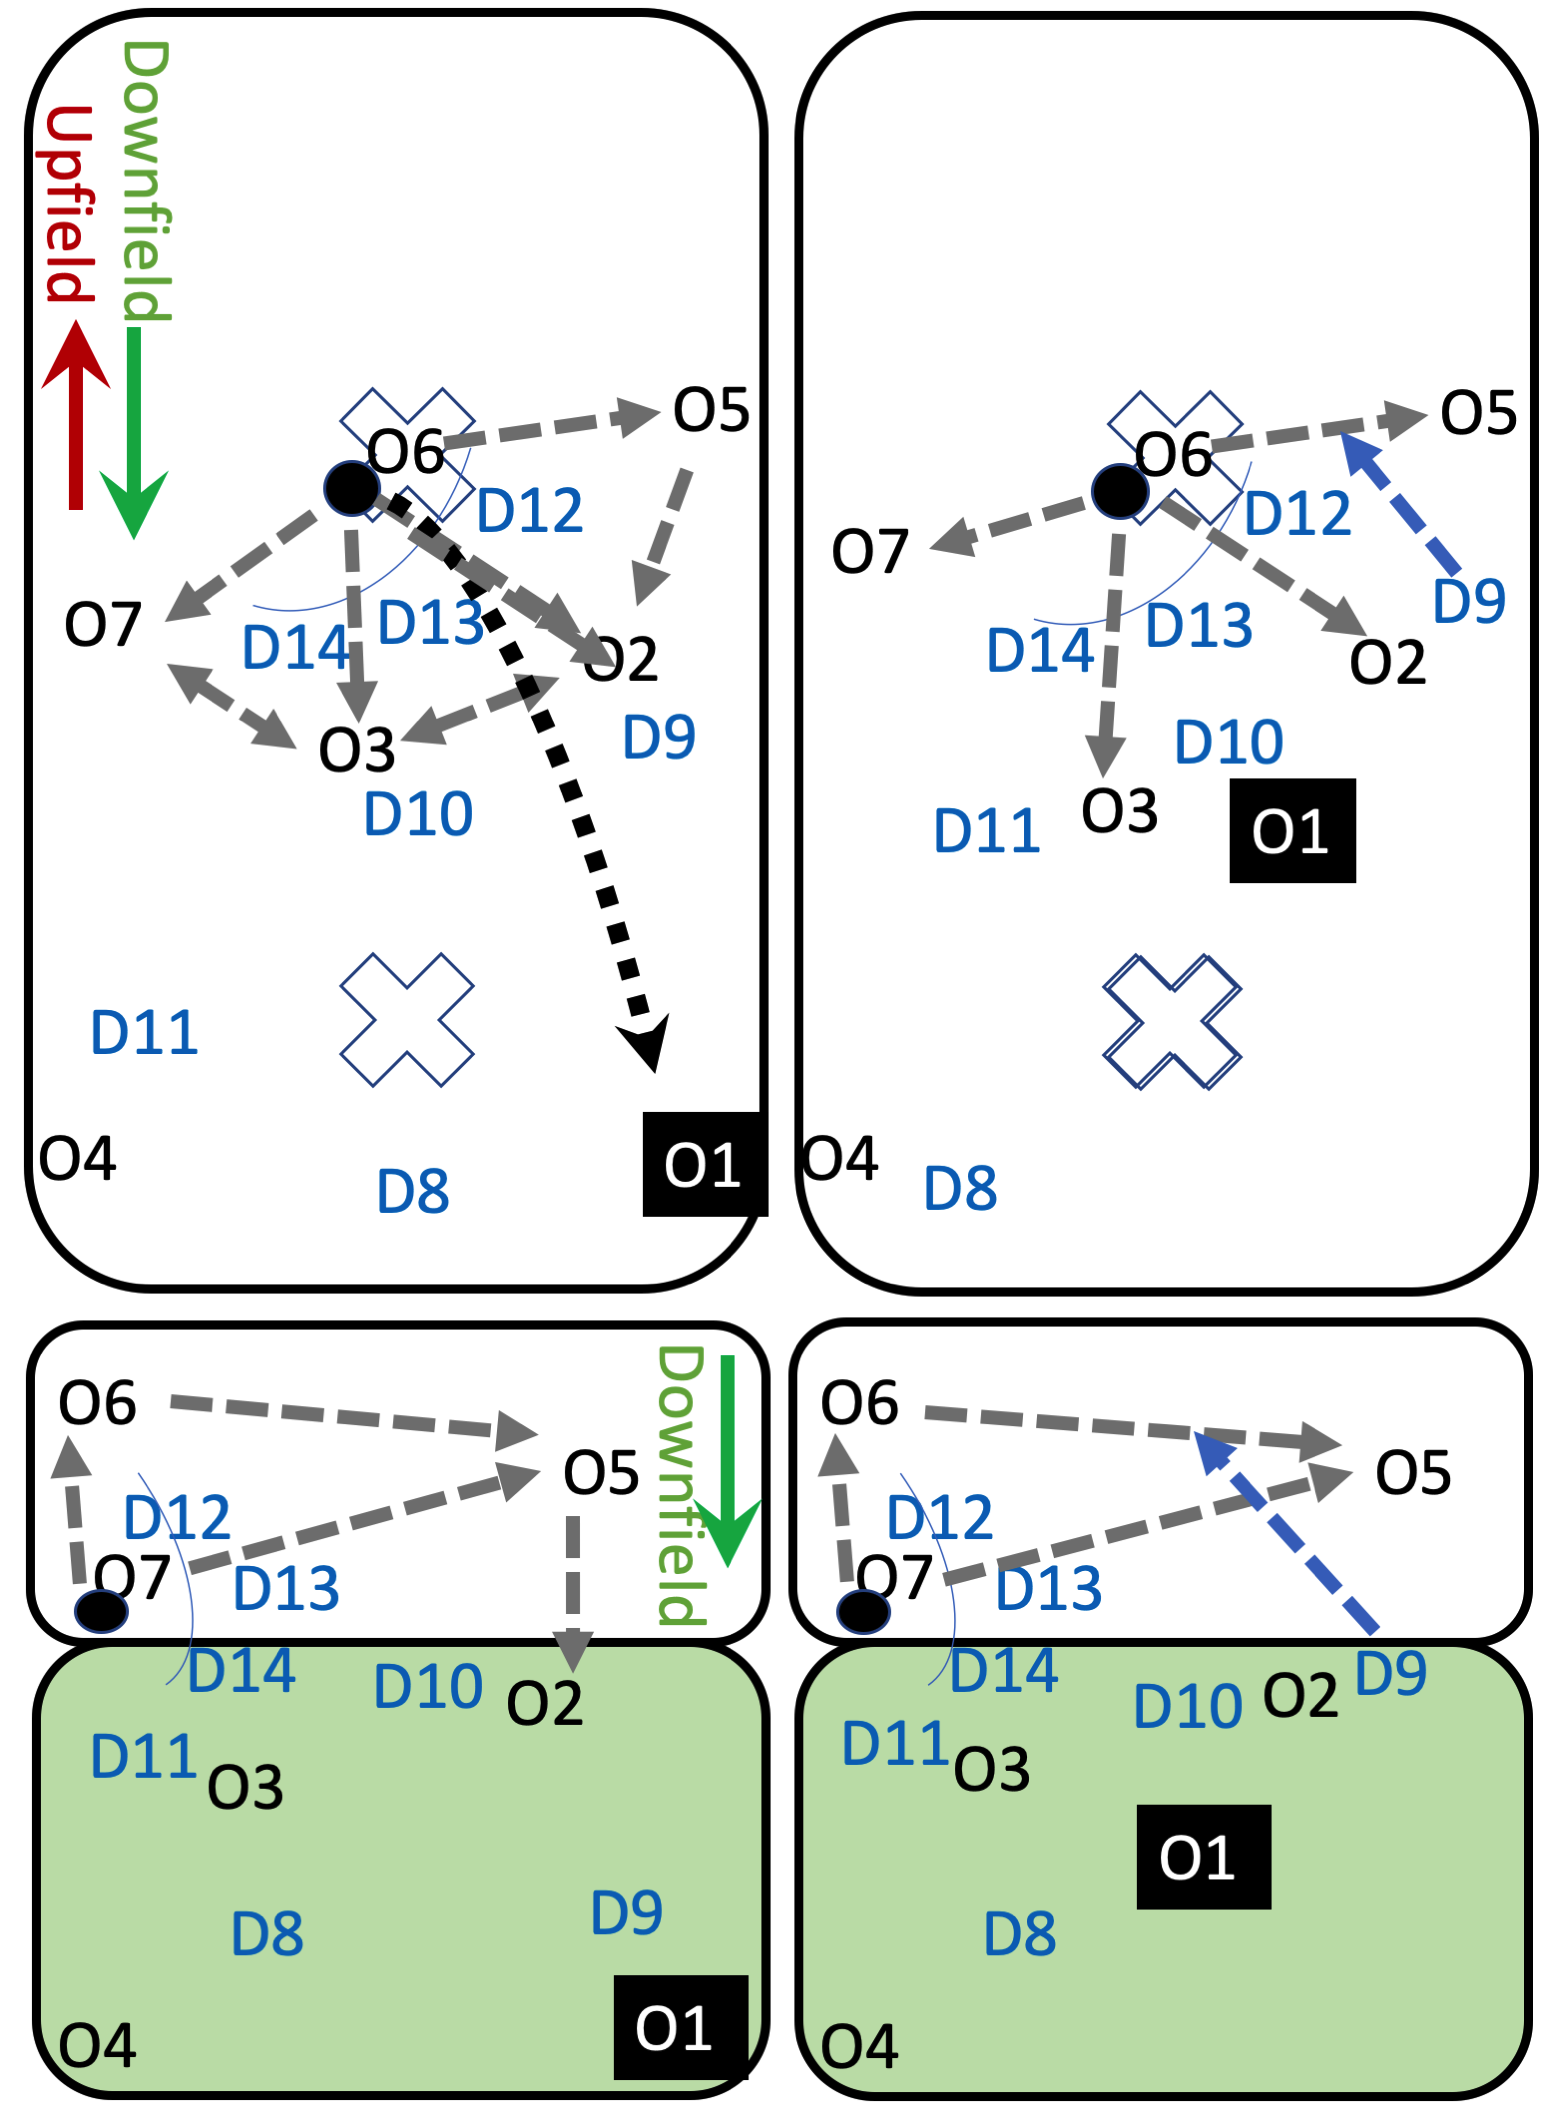
\includegraphics[width=\linewidth]{O1-zone331}
  \caption{331 zone formation}
  \label{fig:O1-zone331}
\end{marginfigure}

Figure \ref{fig:O1-zone331}
shows a standard 
3-3-1 zone, but
regardless of what zone it is,
the three ways to beat it are:
(1) over;
(2) round; or
(3) through. 
As O1 
(left wing), 
you are mostly relevant to 
(1) \smallcaps{over}, 
exploiting the gaps between 
D8 
and D9.
Figure \ref{fig:O1-zone331} shows 
throws from O6 to you:
(1) directly 
using a hammer
or a blade 
to get it there
as quickly as possible.
So stand still, 
and look at O6, or
(2) throwing to A, 
for you to go and get. 

If O6 throws
over or through (to O2 or O3), 
or round (to O5) 
there are various ways 
that you, 
O5, 
O2, and
O3 
might seek to split
D10
and D9\footnote{
For example, 
O6 throws (2) through, 
to O2, 
who can then through to 
O3, 
O5 
or you (O1).}
before the cup 
(D12-14) catch up. 
However, 
once the cup arrives, 
it is best to dump to O6, 
as otherwise 
you are trying to throw to 
one of 4-5 offensive players, 
covered by 7 defenders. 
Dump, 
then move downfield 
to make it 7-on-7 again.

If the defence 
continues to play zone 
once the disc 
gets close to the endzone, 
you (O1) 
and the other wing (O4) 
can go and stand 
on the back corners 
of the endzone.  
A direct throw (1) \smallcaps{over}
to you or O4 will then score. 
But If D9 
or D11 
play person match 
on you 
to prevent this, 
then there will be
more space for O2, 
O3, 
O5, 
O6 and
O7 
to score 
at the front of the endzone. 
\end{document}
